\documentclass{article}
\pdfoutput=1
\usepackage{tikz}
\usetikzlibrary{arrows,automata,backgrounds,calc,chains,fadings,folding,decorations.fractals,decorations.pathreplacing,fit,patterns,positioning,mindmap,shadows,shapes.geometric,shapes.symbols,through,trees,plotmarks}

\newcommand{\charlie}{\texttt{Charlie}}
\newcommand{\cora}{\texttt{Cora}}

\begin{document}

\section*{The overall structure and dependencies of Charlie}

The picture below illustrates the package dependencies in \charlie: the core constrained
higher-order rewriting library used in \cora.  Note that there are no mutual dependencies:
every package only depends on those packages above it that it is connected to; that is, A depends
on B if there is a path from B to A following the arrow directions.  For example,
\texttt{charlie.parser} may use classes from \texttt{charlie.util}, \texttt{charlie.parser.lib}
and \texttt{charlie.types}, but not from (e.g.) \texttt{charlie.smt} or \texttt{charlie.reader}.

\begin{center}
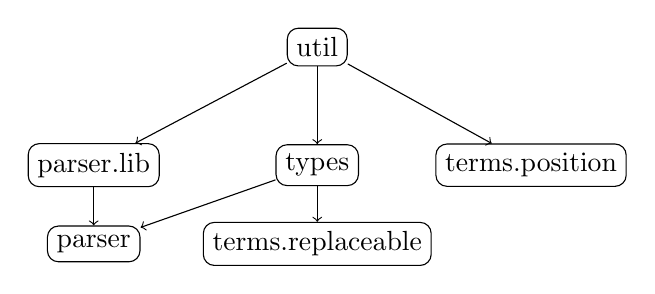
\begin{tikzpicture}[->]
\tikzstyle{veld} = [draw, fill=white, minimum height=0em, minimum width=0em, rounded corners]

\node [veld] (util) {util};

\node [veld] (types) [below of=util, node distance=15mm] {types};
\draw (util) -- (types);

\node [veld] (parserlib) [left of=types, node distance=20mm, anchor=east] {parser.lib};
\draw (util) -- (parserlib);

\node [veld] (parser) [below of=parserlib, node distance=10mm] {parser};
\draw (parserlib) -- (parser);
\draw (types) -- (parser);

\node [veld] (position) [right of=types, node distance=15mm, anchor=west] {terms.position};
\draw (util) -- (position);

\node [veld] (replaceable) [below of=types, node distance=10mm] {terms.replaceable};
\draw (types) -- (replaceable);

%\node [veld] (smt) [right of=position, node distance=17mm, anchor=west] {smt};
%\draw (util) -- (smt);
%
%\node [veld] (terms) [below of=types, node distance=10mm] {terms};
%\draw (types) -- (terms);
%\draw (position) -- (terms);
%
%\node [veld] (trs) [below of=terms, node distance=10mm] {trs};
%\draw (terms) -- (trs);
%
%\node [veld] (smtsolvers) [below of=trs, node distance=10mm] {smtsolvers};
%\draw (parserlib) -- (smtsolvers);
%\draw (smt) -- (smtsolvers);
%
%\node [veld] (reader) [below of=parser, node distance=20mm] {reader};
%\draw (parser) -- (reader);
%\draw (trs) -- (reader);
%
%\node [veld] (theory) [below of=smt, node distance=30mm] {theorytranslation};
%\draw (trs) -- (theory);
%\draw (smt) -- (theory);
\end{tikzpicture}
\end{center}

\newpage
\section{Util}

The util package has no dependencies, and contains general utility classes -- arguably, classes
that could be in the Java library rather than a term rewriting library.

\begin{itemize}
\item \texttt{Either} -- to represent a value that can have one of two possible types
\item \texttt{Pair} -- to represent a value consisting of two underlying values \\\ 

\item \texttt{NullStorageException} -- an exception to be thrown when the user tries to store
  structures in a structure that should not have null elements
\item \texttt{UserException} -- an exception that may need to be shown to the user at some point,
  rather than merely to the programmer
\item \texttt{ExceptionLogger} --- a tool to log exceptions that we don't want to throw, nor
  \emph{necessarily} show to the user \\\ 

\item \texttt{FixedList} -- an immutable list
\item \texttt{FixedSet} -- an immutable set
\item \texttt{LookupMap} -- an immutable map with strings as keys \\\ 

\item \texttt{SystemUtils} -- a class to check information about the current OS
\item \texttt{ProcessCaller} -- a class to call external processes (such as an SMT solver)
\end{itemize}

\end{document}

